\documentclass{article}
\usepackage{multirow}
\usepackage[margin=1in]{geometry}
\usepackage[utf8]{inputenc}
\usepackage{graphicx}
\usepackage{color}
\usepackage{colortbl}
\usepackage{indentfirst}
\usepackage{media9}
\usepackage{listings}
\usepackage{textcomp}
\usepackage{caption}
\usepackage{subcaption}
\usepackage{comment}
\usepackage{hyperref}
\usepackage{booktabs}
\usepackage{amsmath}
\setlength{\parindent}{0pt}
\definecolor{Gray}{gray}{0.9}



\title{ENGN 2920F Lab 1}
\author{David Boles}
\date{}

\begin{document}
\maketitle

Note that all testing was performed at 12 volts with the large disk.

\section*{Open Loop Speed vs Duty Cycle}

The system was tested with various, fixed duty cycle values; once a relatively steady state was reached, the speed measurements (in revolutions per second) were averaged over 50 revolutions. The duty cycle was set as a ratio of the active width to the period (e.g. 1 corresponds to the output being fully low).
\begin{center}
  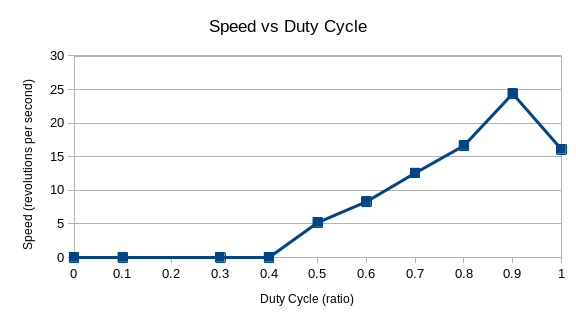
\includegraphics[width=4in]{speed_vs_duty_cycle.png}
\end{center}
As you can see, there's a deadzone below ~40\% duty cycle where the motor doesn't spin the disk. There's also an inconsistency with my 100\% duty cycle datapoint. Unfortunately I didn't notice it at the time so I'm not sure of the source, it's possible I overwrote the data file after storing the measurements or there could be some severe nonlinearities in the system at high duty cycles. The data I have definitely shows that the disk had come up to speed in the range that I averaged it and my software definitely output
a constant low at 100\% duty cycle.



\section*{Pin and Peripheral Configuration}

Pins PD8 and PD9 were configured with the USART 3 peripheral to transmit results to my computer using the board's built-in UART to USB adapter. PE9 was configured with TIMER1 as a 1 kHz PWM output and PE11 was configured as a floating input with interrupts enabled for detecting the rising edges of "encoder info" pulses. TIMER2 was configured to increment roughly 65536 times a second for timing the pulses' period. Finally, PE13 was configured as a push-pull output for debugging interrupt start delay (using semihosting for printing caused issues initially) and to verify that the interrupt completed well before new pulses would arrive.

\section*{PID Controller Tuning}
I tested my PID controller with a step from nearly stopped to a setpoint of 10 revolutions per second. After starting with a constant term that would allow the disk to spin I generally took a three-step approach to tuning my controller: increase $K_P$ until I had a pretty good response with stable, non-excessive oscillations, increase $K_D$ to reduce those oscillations, and finally increase $K_I$ to remove the steady-state error. The first step proceeded fairly well, this was my end result with $K_P = 0.4$ and $C = 0.5$.
\begin{center}
  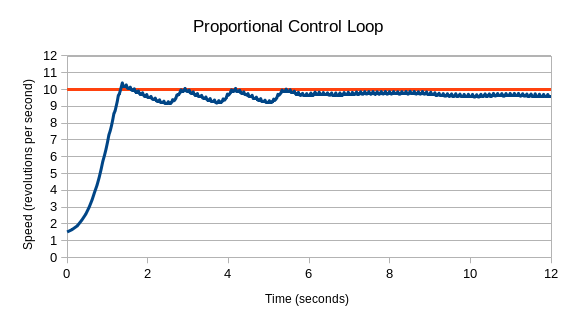
\includegraphics[width=4in]{p_loop.png}
\end{center}
I monitored the PWM output while tuning and, as I increased $K_D$, I noticed that it began to saturate. To prevent that I lowering the other two terms. The feedback ``noise'' (from hall effect sensor and magnet placement variation) was also problematic so I increased the number of pulses per controller update to 24, averaging over every full revolution. I finished with a slightly underdamped response that I was pretty happy with at $K_P = 0.2$, $K_D = 0.03$, and $C = 0.4$
\begin{center}
  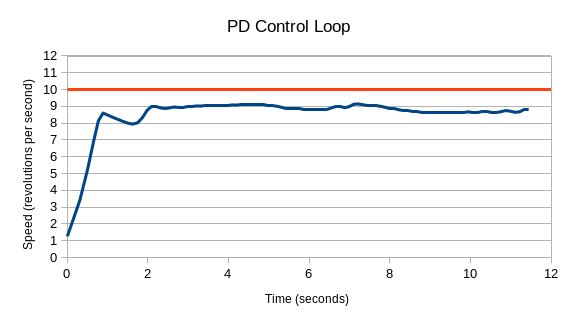
\includegraphics[width=4in]{pd_loop.png}
\end{center}
Finally, by introducing the integral term and doing a little bit more tweaking, I was able to mostly remove the steady-state error. My final values were $K_P = 0.2$, $K_I = 0.007$, $K_D = 0.035$, and $C = 0.3$.
\begin{center}
  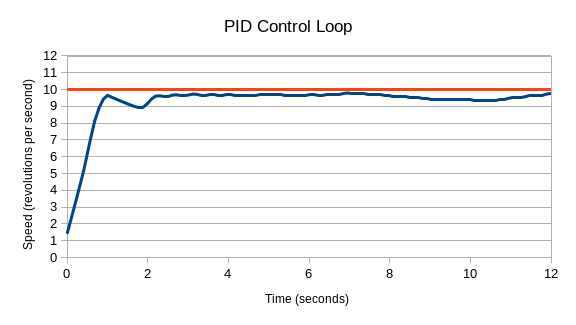
\includegraphics[width=4in]{pid_loop.png}
\end{center}



\section*{Benefits Over Open Loop}

As you can see, the PID controller ramps up more aggressively (about twice as quickly), is likely to get closer to the setpoint (due to the integral term), and oscillates less than an open-loop controller.
\begin{center}
  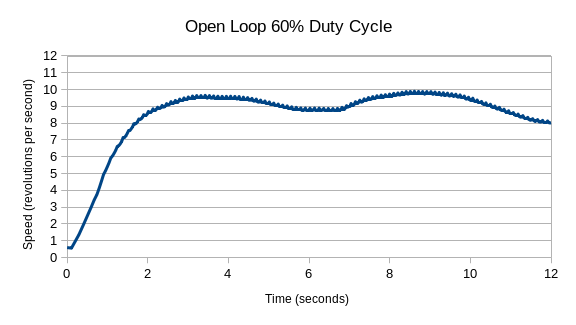
\includegraphics[width=4in]{open_step.png}
\end{center}
The PID controller is also much more resilient to varying or unexpected loads on the system. Unless I added significant resistance, the PID controller kept the disk's speed relatively close to the setpoint. With an open loop controller, it would begin slowing down significantly with even minor resistance.
\begin{center}
  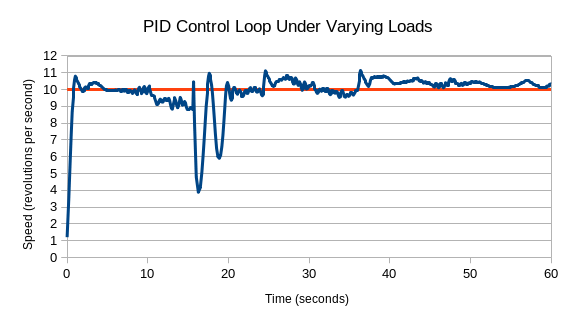
\includegraphics[width=4in]{closed_load.png}
\end{center}
\begin{center}
  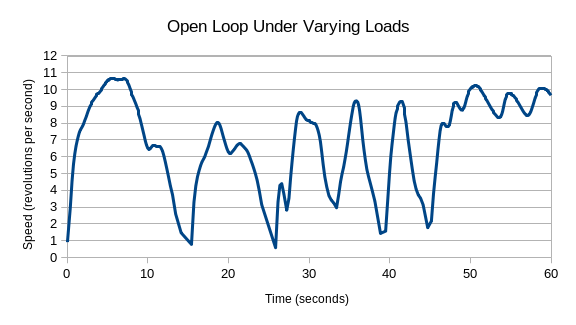
\includegraphics[width=4in]{open_load.png}
\end{center}



\section*{Drawbacks of My Approach}

My controller only updates when a pulse from the controller is recieved. This causes the more trivial yet still significant issue that the controller can't start when the disk is completely still. However, this could be fixed with some minor improvements. The more interesting concern however, which would require a complete redesign, is that not updating at a fixed rate, in addition to having a constant term in the controller, makes mine non-linear. It is therefore hard, if not impossible, to provide any robustness guarantees or to rigorously analyze the performance or stability of the controller. I have therefore decided to write a new implementation using a linear PID controller.




\end{document} 